\subsubsection{Вклад соседней характеристической линии в КДО}
\begin{figure}[H]
  \centering
  \subfloat[$S_1 = 20 $ мкм; $ S_2 = 40$ мкм;]{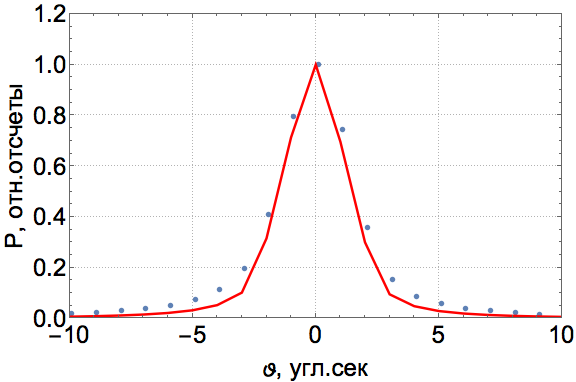
\includegraphics[width=0.45\textwidth]{images/non_disspers_20_40.png}\label{fig:f1}}
  \hfill
  \subfloat[$S_1 = 20 $ мкм; $ S_2 = 40$ мкм; логарифм]{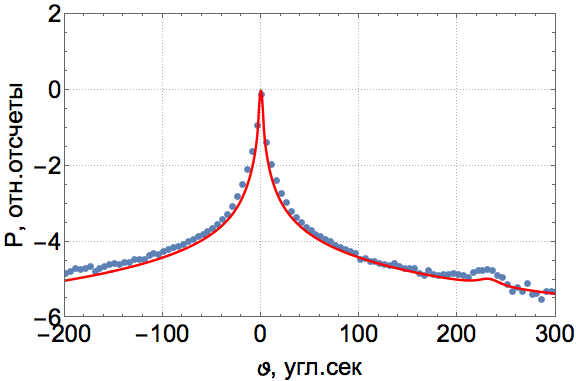
\includegraphics[width=0.45\textwidth]{images/non_disspers_20_40_log.png}\label{fig:f2}}
  \hfill
  \subfloat[$S_1 = 300 $ мкм; $ S_2 = 200$ мкм;]{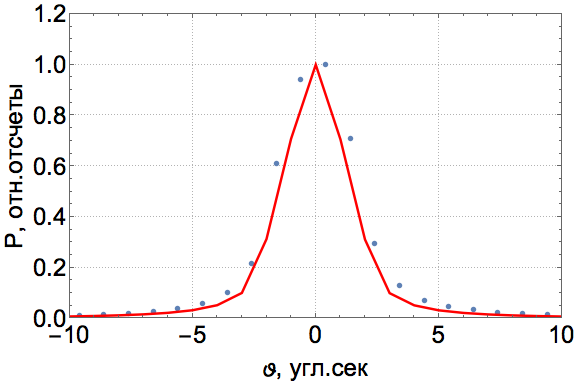
\includegraphics[width=0.45\textwidth]{images/non_disspers_300_200.png}\label{fig:f2}}
  \hfill
  \subfloat[$S_1 = 300 $ мкм; $ S_2 = 200$ мкм; логарифм]{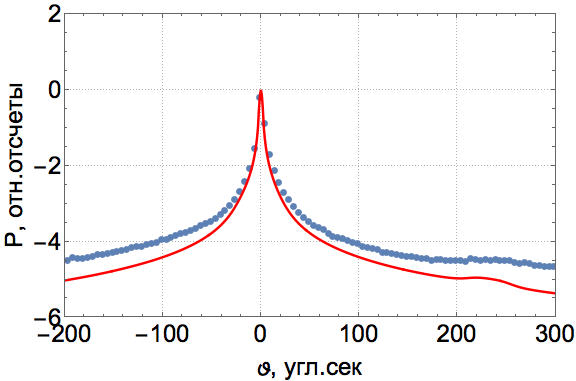
\includegraphics[width=0.45\textwidth]{images/non_disspers_300_200_log.png}\label{fig:f2}}
  \caption{Двухкристальная КДО для схемы с кристаллом монохроматором Si(220) и образцом  Si(440)}
  \label{ris:non_disspers_kdo}
\end{figure}
